\documentclass[11pt,a4paper]{article}
\usepackage[margin=2.5cm]{geometry}
\usepackage{booktabs}
\usepackage{hyperref}
\usepackage{amsmath}
\usepackage{amssymb}
\usepackage{graphicx}
\usepackage{caption}
\usepackage{subcaption}
\usepackage{listings}
\usepackage{xcolor}
\usepackage{natbib}
\usepackage{algorithm}
\usepackage{algpseudocode}
\usepackage{tikz}
\usetikzlibrary{decorations.pathreplacing}
\usepackage{amsthm}
\setlength{\parindent}{0pt}
\setlength{\parskip}{0.5\baselineskip}

\theoremstyle{definition}
\newtheorem{definition}{Definition}
\theoremstyle{plain}
\newtheorem{lemma}{Lemma}

\definecolor{codegreen}{rgb}{0,0.6,0}
\definecolor{codegray}{rgb}{0.5,0.5,0.5}
\definecolor{codepurple}{rgb}{0.58,0,0.82}
\definecolor{backcolour}{rgb}{0.95,0.95,0.92}

\lstdefinestyle{mystyle}{
backgroundcolor=\color{backcolour},
commentstyle=\color{codegreen},
keywordstyle=\color{magenta},
numberstyle=\tiny\color{codegray},
stringstyle=\color{codepurple},
basicstyle=\ttfamily\footnotesize,
breakatwhitespace=false,
breaklines=true,
captionpos=b,
keepspaces=true,
numbers=left,
numbersep=5pt,
showspaces=false,
showstringspaces=false,
showtabs=false,
tabsize=2
}
\lstset{style=mystyle}

\title{\textbf{The Li-Chao Tree: Algorithm Specification and Analysis}}
\author{Li Chao}
\date{\today}

\begin{document}

\maketitle

\begin{abstract}
The Li-Chao tree (LICT) was first introduced in 2012 lecture materials as an efficient data structure for dynamic lower envelope maintenance. In the years since, it has achieved widespread adoption within the competitive programming community, yet no formal specification has appeared in the peer-reviewed literature. This paper provides the definitive formalization of the Li-Chao tree, serving as both the official specification and an expansion of the original 2012 lecture materials. We present complete algorithmic specifications, establish formal correctness proofs, analyze theoretical complexity, and provide empirical performance characterization. The LICT offers distinct advantages in implementation simplicity, numerical stability, and extensibility to advanced variants such as persistence and line segments.
\end{abstract}

\section{Introduction}

Dynamic Lower Envelope maintenance is a fundamental problem in computational geometry with extensive applications. We focus on the Li-Chao tree (LICT), a data structure that maintains a set of linear functions while supporting insertion and query operations. The problem is defined as follows: given a dynamic set of linear functions $y = kx + b$, support efficient insertion of new lines and querying the minimum (or equivalently, maximum) value at arbitrary $x$ coordinates. This report focuses on minimum queries; maximum queries are obtained by negating line parameters.

Formally, we require a data structure supporting two operations:
\begin{enumerate}
\item \textbf{Add Line:} Insert a new line $y = kx + b$ into the structure.
\item \textbf{Query:} Given $x_0$, compute
\[
\min_{i} \{k_i x_0 + b_i\}
\]
over all lines currently in the structure.
\end{enumerate}

The LICT provides pseudo-polynomial $O(\log C)$ time per operation for minimum (or maximum) queries, where
\[
C = \frac{\text{coordinate range}}{\text{precision level}}
\]
represents the ratio of the coordinate range to the precision level.
For integer coordinates with range $[0, 10^9]$, $C = 10^9$; for the same range with precision $10^{-6}$, $C = 10^{15}$.

The structure also supports line segments (lines defined only on finite intervals $[x_l, x_r]$) in addition to infinite lines.

\section{Related Work}\label{sec:related}

Several approaches exist for Dynamic Lower Envelope maintenance, each with distinct trade-offs in terms of time complexity, implementation complexity, and applicability constraints. We review these solutions to establish the context for the LICT.

Dynamic maintenance of geometric configurations has been studied extensively in computational geometry.

\subsection{Overmars and van Leeuwen (1981)}

Overmars and van Leeuwen \cite{overmars1981} presented foundational work on dynamic convex hull maintenance. Their data structure supports insertion and deletion of lines while maintaining the lower envelope, enabling efficient querying of the minimum value at any point.

Their approach uses a balanced binary search tree to explicitly maintain the convex hull. Each node stores a line, and the tree is ordered by slope. Intersection points between adjacent lines are computed to determine the hull structure. Queries take $O(\log n)$ time, while insertions and deletions require $O(\log^2 n)$ time.

\subsection{Monotonic Convex Hull Trick}

The monotonic convex hull trick addresses the special case where line slopes are inserted in monotonically increasing or decreasing order.

When insertions arrive in order of monotonically increasing (or decreasing) slopes, a deque-based approach achieves $O(1)$ amortized time per insertion and $O(1)$ amortized time per query. This variant, widely used in dynamic programming optimization, maintains the convex hull incrementally without requiring balanced tree structures. However, the monotonicity restriction limits its applicability to problems where line slopes are known to follow a specific order.

\subsection{Dynamic Convex Hull Trick}

For arbitrary insertion sequences without monotonicity constraints, a balanced binary search tree maintains the hull explicitly. Each insertion and query requires $O(\log n)$ amortized time. The implementation complexity stems from the need to compute and maintain intersection points between adjacent lines in the hull.

The Dynamic CHT requires computing intersection points between adjacent lines in the hull as
\[
x_{\text{intersect}} = \frac{b_2 - b_1}{k_1 - k_2},
\]
necessitating careful handling of precision (near parallel lines).

\section{Overview}\label{sec:lichao}

This section presents the Li-Chao tree.

\subsection{Core Insight}

The Li-Chao tree is built upon a fundamental observation about line dominance over intervals. Consider two lines defined over an interval $[l, r]$:
\[
f_1(x) = k_1x + b_1 \quad \text{and} \quad f_2(x) = k_2x + b_2.
\]
Since two distinct lines intersect at most once, one line must be strictly lower than the other on more than half of the interval.

Without loss of generality, assume $f_1$ dominates (achieves the lower value) on the majority subinterval $[m, r]$ where
\[
m = \frac{l+r}{2}.
\]
We designate $f_1$ as the \emph{representative} line for $[l, r]$, serving as the optimal answer for any query $x \in [l, m]$.

The key insight is that $f_2$ only requires consideration when the query falls in the minority subinterval $[m, r]$, which comprises at most half the original interval. This observation enables a recursive decomposition: either the query is answered by the current representative, or we recurse on a subproblem of strictly half the size.

This interval-halving property yields the logarithmic query time and forms the basis of the tree structure.

\subsection{Algorithmic Approach}

The LICT offers a fundamentally different approach based on implicit envelope maintenance through interval subdivision. Rather than tracking the convex hull geometry explicitly, the structure maintains the best line at each interval, recursively partitioning the query range.

We first consider the simplest and most common setting: all queried $x$-coordinates are integers. In this case, if the coordinate range is $[0, C-1]$ for some positive integer $C$, the tree recursively bisects this range into subintervals $[l, r]$ where $l, r \in \mathbb{Z}$. Every leaf corresponds to a single integer, so the tree has depth $\lceil \log_2 C \rceil$ and every query lands at a unique leaf. This integer setting is the one most frequently encountered in competitive programming and in many algorithm design applications, and we use it throughout the examples below.

\textbf{Remark (non-integer queries).} The same structure handles queries at non-integer coordinates by refining the discretisation. If queries require precision $\epsilon$ (e.g., $\epsilon = 10^{-6}$), one can rescale the coordinate range by $1/\epsilon$, effectively treating each precision step as one unit. The coordinate universe size becomes $C = \text{coordinate range} / \epsilon$, and the tree depth grows to $\lceil \log_2 C \rceil$ accordingly. All algorithmic details remain identical; only the universe size changes. For example, a range of $[0, 10^9]$ with precision $10^{-6}$ yields $C = 10^{15}$ and tree depth $\approx 50$.

Each node in the tree represents an interval $[l, r]$ and stores one line. 

\paragraph{Insertion.} A line is \emph{routed} through the tree following a single path from root to leaf. At each node on this path, the new line is compared with the currently stored line. The line that achieves the lower value at the midpoint
\[
m = \frac{l+r}{2}
\]
is \emph{stored} at that node; the suboptimal line continues downward to be routed through the appropriate child subtree.

The appropriate child is determined by where the relative ordering changes. Let $f_\text{new}(x) = k_\text{new} x + b_\text{new}$ denote the new line and $f_\text{stored}(x) = k_\text{stored} x + b_\text{stored}$ denote the line currently stored at the node. Define boolean comparison values:
\begin{align*}
L &= [f_\text{new}(l) < f_\text{stored}(l)] \\
M &= [f_\text{new}(m) < f_\text{stored}(m)]
\end{align*}
where $[\cdot]$ denotes 1 if true and 0 if false. The child selection rule is:
\begin{equation*}
\text{child} =
\begin{cases}
\text{left} & \text{if } L \neq M \\
\text{right} & \text{if } L = M
\end{cases}
\end{equation*}
This follows from the single-intersection property: if the ordering changes between $l$ and $m$, the intersection point lies in $[l, m]$; otherwise, it lies in $[m, r]$.

Figure~\ref{fig:insertion-example} illustrates the insertion process with a concrete integer example.

\begin{figure}[h]
\centering
\begin{tikzpicture}[scale=0.85, every node/.style={font=\small}]
% Tree structure on the left
\begin{scope}[xshift=-5cm]
% Root node [0, 8]
\node[draw, rectangle, fill=blue!10, minimum width=2.2cm] (root) at (0,0) {$[0, 8]$: $y=x$};
\node[below=0.1cm of root] {\small $m=4$};

% Level 1 nodes
\node[draw, rectangle, fill=blue!10, minimum width=2.2cm] (l1) at (-2,-2.5) {$[0, 4]$: $y=2x$};
\node[below=0.1cm of l1] {\small $m=2$};
\node[draw, rectangle, minimum width=2.2cm] (r1) at (2,-2.5) {$[4, 8]$: $y=x$};

% Level 2 nodes
\node[draw, rectangle, minimum width=2.2cm] (l2l) at (-3,-5) {$[0, 2]$: $-$};
\node[draw, rectangle, minimum width=2.2cm] (l2r) at (-1,-5) {$[2, 4]$: $-$};
\node[draw, rectangle, fill=red!10, minimum width=2.2cm] (r2l) at (1,-5) {$[4, 6]$: $y=10$};
\node[below=0.1cm of r2l] {\small $m=5$};
\node[draw, rectangle, minimum width=2.2cm] (r2r) at (3,-5) {$[6, 8]$: $-$};

% Edges
\draw[->, thick] (root) -- (l1) node[midway, left] {\small if $L \neq M$};
\draw[->, thick] (root) -- (r1) node[midway, right] {\small if $L = M$};
\draw[->] (l1) -- (l2l);
\draw[->] (l1) -- (l2r);
\draw[->, thick, red] (r1) -- (r2l) node[midway, left, red] {\small new line};
\draw[->] (r1) -- (r2r);
\end{scope}

% Geometric view on the right
\begin{scope}[xshift=3cm]
% Axes
\draw[->] (-0.5,0) -- (9,0) node[right] {$x$};
\draw[->] (0,-0.5) -- (0,10) node[above] {$y$};

% X-axis labels
\foreach \x in {0,2,4,6,8} {
    \draw (\x,0.1) -- (\x,-0.1) node[below] {\x};
}

% Lines
% Line y = x (stored at root, also at [4,8])
\draw[thick, blue] (0,0) -- (8,8) node[right] {$y=x$ (stored at root)};

% Line y = 2x (stored at [0,4], routed to left)
\draw[thick, green!60!black] (0,0) -- (4,8) node[above] {$y=2x$ (stored at $[0,4]$)};

% New line y = 10 (inserted, stored at [4,6])
\draw[thick, red, dashed] (0,10) -- (8,10) node[right] {$y=10$ (new line)};

% Key points
\filldraw[blue] (4,4) circle (2pt);
\node[below right] at (4,4) {\small $(4,4)$};
\filldraw[green!60!black] (2,4) circle (2pt);
\node[above] at (2,4) {\small $(2,4)$};
\filldraw[red] (5,10) circle (2pt);
\node[above] at (5,10) {\small $(5,10)$};
\filldraw[blue] (5,5) circle (2pt);
\node[below] at (5,5) {\small $(5,5)$};

% Interval brackets
\draw[thick, decorate, decoration={brace, amplitude=5pt, mirror}] (0,-1.2) -- (4,-1.2) node[midway, below=8pt] {\small $[0,4]$};
\draw[thick, decorate, decoration={brace, amplitude=5pt, mirror}] (4,-1.2) -- (8,-1.2) node[midway, below=8pt] {\small $[4,8]$};

% Annotations
\node[align=left] at (4,-3.5) {\small \textbf{Step 1:} At root $[0,8]$: $y=2x$ lower at $m=4$?\\
\small No ($8 > 4$), so swap and route to right.\\
\small \textbf{Step 2:} At $[4,8]$: $y=10$ lower at $m=6$?\\
\small No ($10 > 6$), but check $[4,6]$: $y=10$ lower at $m=5$?\\
\small Yes ($10 > 5$), store here.};
\end{scope}
\end{tikzpicture}
\caption{Line Insertion Example. Inserting line $y=10$ into a tree with existing lines $y=x$ and $y=2x$. The new line is compared at each node; since it is higher at midpoints, it gets routed right until finding its optimal interval $[4,6]$.}
\label{fig:insertion-example}
\end{figure}

Algorithms~\ref{alg:insert} and~\ref{alg:query} present the insertion and query procedures.

When the insertion reaches maximum depth ($r - l < \epsilon$, where $\epsilon$ is the required precision), the interval is too narrow to distinguish any two query points. The stored line already resolves every query in that interval, so the losing line is simply dropped: no further recursion is needed. For integer coordinates ($\epsilon = 1$), this condition simplifies to $l = r$.

\begin{algorithm}[h]
\caption{LICT Line Insertion}
\label{alg:insert}
\begin{algorithmic}[1]
\Require Node pointer $node$, new line $new\_line$, interval $[l, r]$
\If{$node$ is null}
\State $node \gets \text{new Node}(new\_line)$
\State \Return
\EndIf
\State $m \gets l + (r - l) / 2$
\State $lef \gets new\_line.eval(l) < node.line.eval(l)$
\State $midf \gets new\_line.eval(m) < node.line.eval(m)$
\If{$midf$}
\State swap($node.line$, $new\_line$)
\EndIf
\If{$r - l < \epsilon$} \Comment{Max depth reached; drop the losing line}
\State \Return
\EndIf
\If{$lef \neq midf$}
\State \Call{Insert}{$node.left$, $new\_line$, $l$, $m$}
\Else
\State \Call{Insert}{$node.right$, $new\_line$, $m$, $r$}
\EndIf
\end{algorithmic}
\end{algorithm}

\begin{figure}[h]
\centering
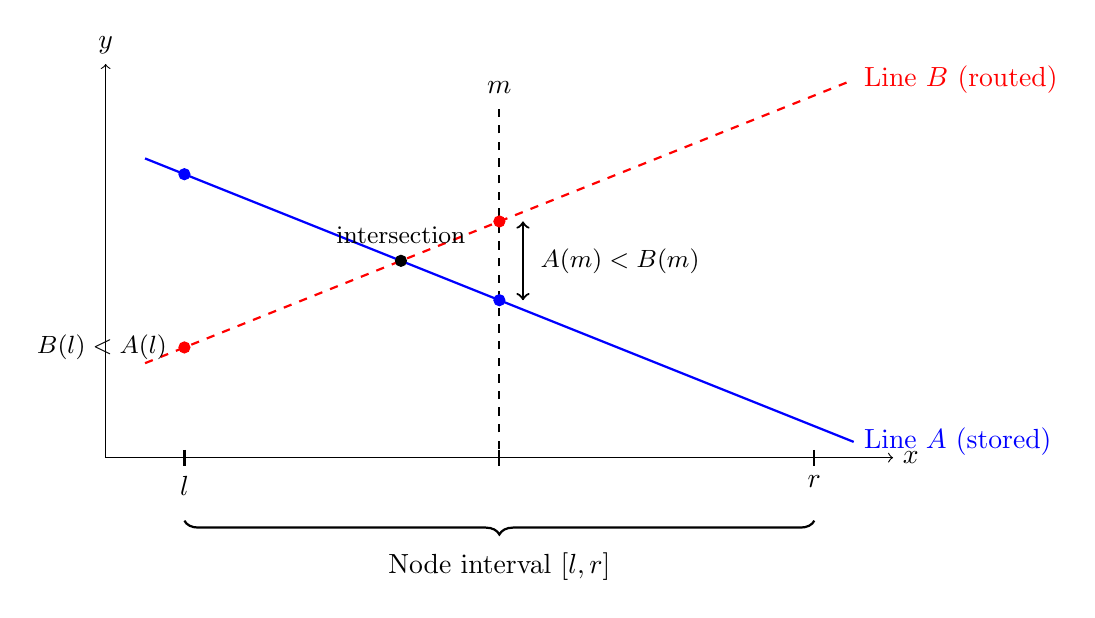
\begin{tikzpicture}[scale=1.0]
% Draw axes
\draw[->] (0,0) -- (10,0) node[right] {$x$};
\draw[->] (0,0) -- (0,5) node[above] {$y$};

% Draw interval [l, r] on x-axis
\draw[thick] (1,0.1) -- (1,-0.1) node[below] {$l$};
\draw[thick] (9,0.1) -- (9,-0.1) node[below] {$r$};
\draw[thick, decorate, decoration={brace, amplitude=5pt, mirror}] (1,-0.8) -- (9,-0.8) node[midway, below=8pt] {Node interval $[l, r]$};

% Draw midpoint
\draw[thick, dashed] (5,-0.1) -- (5,4.5) node[above] {$m$};
\draw[thick] (5,0.1) -- (5,-0.1);

% Draw two intersecting lines
% Line A: y = -0.4x + 4 (stored at node - lower at midpoint, higher at left)
\draw[thick, blue] (0.5,3.8) -- (9.5,0.2) node[right] {Line $A$ (stored)};
% Line B: y = 0.4x + 1 (routed to left child - lower at left, higher at mid)
\draw[thick, red, dashed] (0.5,1.2) -- (9.5,4.8) node[right] {Line $B$ (routed)};

% Mark intersection point (at x = 3.75)
\filldraw[black] (3.75,2.5) circle (2pt);
\node[above] at (3.75,2.6) {\small intersection};

% Mark values at midpoint (x = 5)
\filldraw[blue] (5,2.0) circle (2pt);
\filldraw[red] (5,3.0) circle (2pt);
\draw[thick, <->] (5.3,2.0) -- (5.3,3.0);
\node[right] at (5.4,2.5) {\small $A(m) < B(m)$};

% Mark values at left endpoint (x = 1)
\filldraw[blue] (1,3.6) circle (2pt);
\filldraw[red] (1,1.4) circle (2pt);
\node[left] at (0.9,1.4) {\small $B(l) < A(l)$};
\end{tikzpicture}
\caption{Interval Advantage Line Diagram. The node stores Line $A$ because it achieves the lower value at the midpoint. Line $B$ is routed to the left child where it may be optimal.}
\label{fig:interval-advantage}
\end{figure}

Note that this is \emph{local} optimality only. Lines routed down other branches may achieve lower values at the midpoint, so the stored line is not necessarily globally optimal at that coordinate.

\paragraph{Query.} We traverse the path to $x_0$, evaluating all stored lines along the path. The minimum value encountered equals the lower envelope at $x_0$ because any line that could be optimal at $x_0$ is stored on this path.

Figure~\ref{fig:query-example} illustrates the query process with a concrete integer example.

\begin{figure}[h]
\centering
\begin{tikzpicture}[scale=0.85, every node/.style={font=\small}]
% Tree structure on the left
\begin{scope}[xshift=-5cm]
% Root node [0, 8]
\node[draw, rectangle, fill=blue!10, minimum width=2.2cm] (root) at (0,0) {$[0, 8]$: $y=x$};
\node[below=0.1cm of root] {\small $m=4$};

% Level 1 nodes
\node[draw, rectangle, fill=green!10, minimum width=2.2cm] (l1) at (-2,-2.5) {$[0, 4]$: $y=2x$};
\node[below=0.1cm of l1] {\small $m=2$};
\node[draw, rectangle, minimum width=2.2cm] (r1) at (2,-2.5) {$[4, 8]$: $y=x$};

% Level 2 nodes
\node[draw, rectangle, fill=yellow!20, minimum width=2.2cm] (l2l) at (-3,-5) {$[0, 2]$: $-$};
\node[draw, rectangle, minimum width=2.2cm] (l2r) at (-1,-5) {$[2, 4]$: $-$};
\node[draw, rectangle, minimum width=2.2cm] (r2l) at (1,-5) {$[4, 6]$: $y=10$};
\node[draw, rectangle, minimum width=2.2cm] (r2r) at (3,-5) {$[6, 8]$: $-$};

% Query path highlighted
\draw[->, very thick, blue] (root) -- (l1);
\draw[->, very thick, blue] (l1) -- (l2l);

% Query point annotation
\node[circle, draw, red, thick, minimum size=0.5cm] at (-3,-5) {};
\node[below=0.3cm of l2l, red] {\small Query $x=1$};

% Legend
\node[align=left] at (0,-7) {\small \textbf{Query path:} $[0,8] \to [0,4] \to [0,2]$\\
\small Lines evaluated: $y=x$, $y=2x$};
\end{scope}

% Geometric view on the right
\begin{scope}[xshift=3cm]
% Axes
\draw[->] (-0.5,0) -- (9,0) node[right] {$x$};
\draw[->] (0,-0.5) -- (0,10) node[above] {$y$};

% X-axis labels
\foreach \x in {0,2,4,6,8} {
    \draw (\x,0.1) -- (\x,-0.1) node[below] {\x};
}

% Query line at x=1
\draw[thick, red, dashed] (1,-0.5) -- (1,10) node[above] {Query $x=1$};

% Lines
% Line y = x (stored at root)
\draw[thick, blue] (0,0) -- (8,8) node[right] {$y=x$};

% Line y = 2x (stored at [0,4])
\draw[thick, green!60!black] (0,0) -- (4,8) node[above] {$y=2x$};

% Line y = 10 (stored at [4,6])
\draw[thick, orange] (4,10) -- (6,10);

% Evaluate at x=1
\filldraw[blue] (1,1) circle (2.5pt);
\node[below right] at (1,1) {\small $y=x$ gives $1$};
\filldraw[green!60!black] (1,2) circle (2.5pt);
\node[above right] at (1,2) {\small $y=2x$ gives $2$};

% Minimum indicator
\draw[thick, ->, red] (1.5,0.5) -- (1.1,0.9);
\node[right] at (1.5,0.5) {\small \textbf{Minimum:} $1$};

% Evaluation table
\node[draw, rectangle, fill=white] at (4,-2.5) {
\begin{tabular}{l|c}
\textbf{Line} & \textbf{Value at $x=1$} \\
\hline
$y=x$ & $1$ \\
$y=2x$ & $2$ \\
$y=10$ & $10$ (not on path) \\
\hline
\textbf{Result} & $\min = 1$
\end{tabular}
};
\end{scope}
\end{tikzpicture}
\caption{Query Example. Querying at $x=1$ traverses the path $[0,8] \to [0,4] \to [0,2]$, evaluating stored lines $y=x$ and $y=2x$. The minimum value $1$ is returned. Line $y=10$ is not evaluated because it is stored in a disjoint subtree.}
\label{fig:query-example}
\end{figure}

\begin{algorithm}[h]
\caption{LICT Query}
\label{alg:query}
\begin{algorithmic}[1]
\Require Node pointer $node$, query coordinate $x$, interval $[l, r]$
\Ensure Minimum value at coordinate $x$
\If{$node$ is null}
\State \Return $+\infty$
\EndIf
\State $m \gets l + (r - l) / 2$
\State $val \gets node.line.eval(x)$
\If{$r - l < \epsilon$}
\State \Return $val$
\EndIf
\If{$x \leq m$}
\State \Return $\min(val, \text{\Call{Query}{$node.left$, $x$, $l$, $m$}})$
\Else
\State \Return $\min(val, \text{\Call{Query}{$node.right$, $x$, $m$, $r$}})$
\EndIf
\end{algorithmic}
\end{algorithm}

\subsection{Theoretical Analysis}

We now present a formal analysis of the LICT's correctness and complexity.

\begin{definition}[Coordinate Universe]
The LICT operates on a discrete domain where
\[
C = \frac{\text{coordinate range}}{\text{precision level}}.
\]
The tree depth is $h = \lceil \log_2 C \rceil$.
\end{definition}

\subsubsection{Correctness}

% TODO: create lean formatted code to rewrite the statement here

% Note for Chao: review this carefully

We first establish the geometric intuition underlying the LICT's correctness. The key insight is that two distinct lines intersect at most once. This fundamental property of linear functions ensures that if a line yields a higher value at a midpoint, it can yield a lower value than the stored line on at most one side of the midpoint, never both.

\textbf{Why this maintains the lower envelope.} Consider two lines $A$ and $B$ compared at a node's midpoint $m$:
\begin{itemize}
\item If $A$ achieves a lower value than $B$ at $m$, but $B$ yields a lower value at one endpoint, then $B$ can only outperform $A$ on the side of $m$ containing that endpoint (since two lines intersect at most once).
\item Therefore, $B$ is routed to exactly one child, the side where it might achieve a lower value.
\end{itemize}

This property guarantees that the suboptimal line need only be propagated down a single child path.

\begin{lemma}[Local Optimality Invariant]\label{lem:local-opt}
For any node $v$ with interval $[l, r]$ and midpoint
\[
m = \left\lfloor\frac{l+r}{2}\right\rfloor,
\]
the line stored at $v$ achieves the minimum value at $x = m$ among all lines that have been routed through $v$.
\end{lemma}

\begin{proof}
We proceed by induction on the sequence of insertions.

\textbf{Base case:} When the first line is inserted, it is stored at the root and all descendants are null. The invariant holds trivially.

\textbf{Inductive step:} Assume the invariant holds before inserting a new line $L_{\text{new}}$. Consider the insertion path from root to leaf. At each node $v$ along this path:
\begin{enumerate}
\item Let $L_{\text{stored}}$ be the line currently at $v$.
\item If $L_{\text{new}}(m) \geq L_{\text{stored}}(m)$, we keep $L_{\text{stored}}$ and route $L_{\text{new}}$ to a child. The invariant at $v$ remains satisfied.
\item If $L_{\text{new}}(m) < L_{\text{stored}}(m)$, we swap the lines, storing $L_{\text{new}}$ and routing $L_{\text{stored}}$ to a child. The invariant at $v$ is now satisfied by $L_{\text{new}}$.
\end{enumerate}
The routed line proceeds to exactly one child (determined by the intersection point location), so the inductive hypothesis applies to subtrees. By induction, the invariant holds after all insertions.
\end{proof}

\begin{lemma}[Query Correctness]\label{lem:query-correct}
For any query point $x_0 \in X$, the value returned by the query operation equals $\min_{i} \{k_i x_0 + b_i\}$ over all lines in the structure.
\end{lemma}

\begin{proof}
Consider any line $L$ in the structure and the query point $x_0$. Let $P$ be the unique root-to-leaf path whose intervals all contain $x_0$. Line $L$ follows exactly one root-to-leaf path $P_L$ during insertion.

We claim $L$ is evaluated at $x_0$ if and only if $x_0$ lies in the interval where $L$ is optimal among lines routed through some node on $P_L$. There are two cases:
\begin{enumerate}
\item If $P_L = P$, then $L$ is stored at some node on $P$ (specifically, at the deepest node where it achieved minimum at the midpoint), and is evaluated during the query.
\item If $P_L \neq P$, let $v$ be the deepest node common to both paths. Since $x_0$ is not in the child interval that $L$ was routed to, $x_0$ lies on the opposite side of the midpoint from where $L$ could potentially be better than the stored line. By the single-intersection property of lines, $L$ cannot be optimal at $x_0$.
\end{enumerate}
Thus, exactly those lines that could be optimal at $x_0$ are evaluated, and the minimum over evaluated lines equals the global minimum.
\end{proof}

\subsubsection{Complexity Analysis}

\begin{lemma}[Time Complexity]\label{lem:time-complexity}
Both insertion and query operations require $O(\log C)$ time.
\end{lemma}

\begin{proof}
The LICT is a binary tree of depth
\[
h = \lceil \log_2 C \rceil = O(\log C).
\]

For insertion: The new line follows exactly one root-to-leaf path. At each node, we perform: (1) $O(1)$ line evaluations ($kx + b$); (2) $O(1)$ comparisons; and (3) optionally a line swap. Each operation takes $O(1)$ time. With $O(\log C)$ nodes visited, total time is $O(\log C)$.

For query: The traversal follows one root-to-leaf path with $O(1)$ work per node (line evaluation and comparison). Total time is $O(\log C)$.
\end{proof}

\begin{lemma}[Space Complexity]\label{lem:space-complexity}
The LICT stores at most $O(n \log C)$ nodes in the worst case, where $n$ is the number of inserted lines.
\end{lemma}

\begin{proof}
Each line insertion creates at most one new node per level along its insertion path (when reaching a null child). The path length is
\[
O(\log C).
\]
With $n$ insertions, the total number of nodes is at most $O(n \log C)$.
\end{proof}

\textbf{Deletion.} The standard LICT does not support efficient deletion. Removing a line would require traversing all nodes where that line might be stored and recomputing optimal lines from descendants, which requires $\Omega(n)$ time in the worst case. For applications requiring deletion, an alternative approach is reconstructing the tree periodically.

The LICT's complexity depends on the coordinate range rather than the number of lines. This provides consistent performance regardless of hull size, though it cannot exploit cases where the hull remains small relative to the number of insertions.

\section{Benchmarks}\label{sec:benchmarks}

Reference implementations and benchmarks are available at \url{https://github.com/chnlich/lichao-tree}.

To validate the theoretical complexity analysis and characterize practical performance differences between the LICT and Dynamic CHT, we conducted systematic empirical evaluation across varying problem scales and input distributions.

\subsection{Experimental Setup}

All benchmarks were conducted with the following configuration.

\textbf{Hardware Specifications:}
\begin{itemize}
\item \textbf{CPU:} AMD Ryzen 9 3950X 16-Core Processor @ 3.50GHz (Zen 2 microarchitecture)
\item \textbf{Core Configuration:} 16 cores, 32 threads (SMT enabled)
\item \textbf{L1 Cache:} 512 KiB L1 data cache, 512 KiB L1 instruction cache
\item \textbf{L2 Cache:} 8 MiB
\item \textbf{L3 Cache:} 16 MiB (shared)
\item \textbf{Memory:} 64 GB DRAM
\item \textbf{Platform:} Linux x86\_64 (WSL2 virtualized)
\end{itemize}

\textbf{Software Configuration:}
\begin{itemize}
\item \textbf{Compiler:} g++ 11.4.0
\item \textbf{Optimization Flags:} \texttt{-O3 -std=c++17 -Wall -Wextra}
\item \textbf{Operating System:} Ubuntu 22.04.5 LTS (WSL2, kernel 6.6.87)
\end{itemize}

\textbf{Experimental Parameters:}
\begin{itemize}
\item \textbf{Test sizes:} $10^5$, $10^6$, and $10^7$ operations
\item \textbf{Coordinate range:}
\[
C = 10^9
\]
(assuming integer precision $\epsilon = 1$), with $x, k, m \in [-10^9, 10^9]$
\item \textbf{Random seed:} 42
\item \textbf{Measurement protocol:} Each test was run 10 times; reported times are the average. Variance was low ($<5\%$ coefficient of variation across runs). Benchmarks were run on an isolated system with no other user processes to minimize timing noise.
\item \textbf{Distributions:} We write
\[
X \sim U(a, b)
\]
to denote that random variable $X$ is drawn from a continuous uniform distribution over the interval $[a, b]$.
\begin{itemize}
\item \textbf{Random:} Slopes $k \sim U(-10^9, 10^9)$, intercepts $m \sim U(-10^9, 10^9)$. Expected hull size:
\[
\Theta(\sqrt{n}).
\]
\item \textbf{All on Hull:} Lines $y = i \cdot x - i^2$ for $i \in [1, n]$. All $n$ lines contribute to the hull.
\end{itemize}
\end{itemize}

\subsection{Results}

Table~\ref{tab:results} presents the performance comparison.

\begin{table}[h]
\centering
\caption{Performance Comparison (Time in milliseconds)}
\label{tab:results}
\begin{tabular}{@{}cccc@{}}
\toprule
\textbf{N} & \textbf{Distribution} & \textbf{LICT} & \textbf{Dynamic CHT} \\
\midrule
$10^5$ & Random & 5.0 ms & 3.0 ms \\
$10^5$ & All on Hull & 16.9 ms & 16.0 ms \\
\midrule
$10^6$ & Random & 52.9 ms & 31.3 ms \\
$10^6$ & All on Hull & 693.3 ms & 882.2 ms \\
\midrule
$10^7$ & Random & 548.8 ms & 326.9 ms \\
$10^7$ & All on Hull & 14702.5 ms & 16249.0 ms \\
\bottomrule
\end{tabular}
\end{table}

\subsection{Parameter-Matched Comparison: The $N = C$ Regime}

The theoretical complexity analysis reveals that Dynamic CHT achieves $O(\log n)$ time while LICT achieves $O(\log C)$. To directly compare these regimes, we conduct experiments where the number of lines $N$ equals the coordinate universe size $C$. This configuration mirrors dynamic programming optimizations common in competitive programming, where the state recurrence takes the form:
\[
dp[i] = \min_{0 \le j < i} \{ dp[j] + \text{cost}(j, i) \}
\]
Here, $\text{cost}(j, i)$ represents a linear function of $i$. Since the queries (indices $i$) are within a fixed range $[0, N]$, the coordinate universe size $C$ effectively equals $N$.

In this static universe setting, an iterative segment tree implementation (often called ZKW segment tree) can be employed to reduce recursion overhead and improve cache locality. We therefore include a third variant, \textbf{ZKW LICT}, in this comparison to evaluate the benefits of this specialized optimization against the standard LICT and Dynamic CHT.

\begin{itemize}
\item \textbf{Configuration:} $N = C = 10^5$, $N = C = 10^6$, and $N = C = 10^7$
\item \textbf{Lines:} $k, b \sim U(-C/2, C/2)$
\item \textbf{Query points:} $x \sim U(-C/2, C/2)$
\item \textbf{Operation mix:} $N/2$ insertions followed by $N/2$ queries
\end{itemize}


\begin{table}[h]
\centering
\caption{Performance in $N = C$ Regime (Time in milliseconds)}
\label{tab:nc-regime}
\begin{tabular}{@{}cccccc@{}}
\toprule
\textbf{N = C} & \textbf{Distribution} & \textbf{Algorithm} & \textbf{Insert (ms)} & \textbf{Query (ms)} & \textbf{Total (ms)} \\
\midrule
$10^5$ & Random & LICT & 2.23 & 1.00 & 3.22 \\
$10^5$ & Random & ZKW LICT & 2.39 & 0.59 & 2.98 \\
$10^5$ & Random & Dynamic CHT & 2.15 & 0.36 & 2.51 \\
$10^5$ & All on Hull & LICT & 8.05 & 5.73 & 13.78 \\
$10^5$ & All on Hull & ZKW LICT & 5.41 & 1.93 & 7.34 \\
$10^5$ & All on Hull & Dynamic CHT & 8.86 & 7.69 & 16.54 \\
\midrule
$10^6$ & Random & LICT & 26.77 & 9.89 & 36.65 \\
$10^6$ & Random & ZKW LICT & 27.50 & 6.60 & 34.10 \\
$10^6$ & Random & Dynamic CHT & 23.49 & 3.61 & 27.10 \\
$10^6$ & All on Hull & LICT & 174.34 & 246.87 & 421.20 \\
$10^6$ & All on Hull & ZKW LICT & 83.63 & 66.59 & 150.22 \\
$10^6$ & All on Hull & Dynamic CHT & 259.19 & 346.92 & 606.11 \\
\midrule
$10^7$ & Random & LICT & 314.03 & 104.11 & 418.13 \\
$10^7$ & Random & ZKW LICT & 328.50 & 80.27 & 408.77 \\
$10^7$ & Random & Dynamic CHT & 230.87 & 45.14 & 276.01 \\
$10^7$ & All on Hull & LICT & 4683.66 & 5762.05 & 10445.72 \\
$10^7$ & All on Hull & ZKW LICT & 1724.87 & 1435.00 & 3159.87 \\
$10^7$ & All on Hull & Dynamic CHT & 6738.87 & 7096.22 & 13835.08 \\
\bottomrule
\end{tabular}
\end{table}

\subsection{Analysis}

In the case that $C$ is larger than $N$, both algorithms have similar performance, even if the theoretical complexity of LICT is worse than Dynamic CHT. This is because the $O(\log C)$ factor is small enough to be negligible compared to the $O(\log n)$ factor, while the constant factor of LICT is smaller than that of Dynamic CHT.

In the $N = C$ regime, the ZKW LICT variant demonstrates substantial gains over both alternatives on dense hull inputs, with the $N = C = 10^7$ all-on-hull benchmark completed approximately $4\times$ faster than Dynamic CHT. 

The LICT's division-free operations ensure consistent numerical accuracy across all inputs. For applications involving floating-point coordinates or extreme value ranges, the LICT provides robustness guarantees that the Dynamic CHT by avoiding intersection point computation.

\section{Conclusion}\label{sec:discussion}

The LICT is the preferred choice in the following scenarios:

\subsection{Advantages}

\textbf{Line segment support required.} When the problem involves line segments (lines valid only on subranges) rather than infinite lines, the LICT provides natural $O(\log^2 C)$ insertion. The Dynamic CHT can support segments but requires significantly more complex machinery.

\textbf{Persistence required.} Path copying in the LICT is straightforward: insertions modify only nodes along a single root-to-leaf path, so copying those nodes creates a new version sharing unmodified subtrees with the previous version. Achieving persistence in the Dynamic CHT is substantially more complex due to the need to maintain hull invariants across versions.

\textbf{Near parallel lines.} When working on lines with subtle slope differences, the LICT's division-free operations avoid numerical instability.

\textbf{Implementation time constraints.} In settings such as competitive programming where implementation speed matters, the LICT's simplicity offers a clear advantage. The reduced code size and elimination of geometric corner cases allow for faster, more confident implementation.

\subsection{Limitations}

The LICT has several limitations that affect its applicability:

\textbf{No efficient deletion.} As noted above, the standard LICT does not support deletion of individual lines. Removing a line would require traversing all nodes where that line might be stored and recomputing optimal lines from descendants, requiring $\Omega(n)$ time in the worst case.

\textbf{Coordinate range dependency.} The LICT's complexity depends on $C$, the coordinate range divided by precision. For very large coordinate ranges with fine precision (e.g., 64-bit floating-point values spanning the entire representable range), $C$ can become impractically large.

\subsection{Future Work}

Several directions for future research and development remain:

\textbf{Deletion support.} Developing an efficient deletion mechanism for the LICT would extend its applicability to dynamic scenarios requiring removal of lines. Potential approaches include lazy deletion with periodic reconstruction or augmenting nodes with additional structure to support efficient line removal.

\textbf{Cache-efficient variants.} The LICT's pointer-based tree structure exhibits poor cache locality compared to array-based representations. Investigating cache-oblivious or cache-aware variants could improve practical performance without sacrificing asymptotic guarantees.

\textbf{Parallel implementations.} The LICT's tree structure naturally supports parallel queries, but insertions are inherently sequential. Developing concurrent LICT variants that support parallel insertions while maintaining correctness would benefit multi-core applications.

\textbf{Higher-dimensional extensions.} While the LICT extends naturally to higher dimensions (maintaining hyperplanes instead of lines), the space and time complexities grow exponentially with dimension. Investigating approximate variants or dimensionality reduction techniques could broaden applicability.

\begin{thebibliography}{9}

\bibitem{overmars1981}
Overmars, M.H. and van Leeuwen, J.
\newblock Maintenance of configurations in the plane.
\newblock \emph{Journal of Computer and System Sciences}, 23(2):166 to 204, 1981.

\bibitem{aggarwal1987}
Aggarwal, A. and Tokuyama, T.
\newblock Consecutive interval query and dynamic programming on intervals.
\newblock \emph{Discrete Applied Mathematics}, 20(1):1 to 11, 1988.

\bibitem{zjoi2012}
Li Chao.
\newblock Lecture materials.
\newblock China, 2012.

\bibitem{cp-algorithms}
CP-Algorithms.
\newblock Li-Chao tree.
\newblock \url{https://cp-algorithms.com/geometry/li_chao_tree.html}, 2024.
\newblock Accessed: 2025-02-06.

\bibitem{codeforces}
I\_LOVE\_TIGER.
\newblock Li-Chao tree Tutorial.
\newblock \url{https://codeforces.com/blog/entry/51275}, 2017.
\newblock Accessed: 2025-02-06.

\bibitem{kactl}
KTH Algorithm Library (KACTL).
\newblock LineContainer.
\newblock \url{https://github.com/kth-competitive-programming/kactl}, 2024.
\newblock Accessed: 2025-02-06.

\end{thebibliography}

\end{document}
